\documentclass[11pt,letterpaper]{article}

%%%%%%%%%%%%%%%%%%%%%%%%%%%%%%                               
\pagestyle{plain}                                                      %%
%%%%%%%%%% EXACT 1in MARGINS %%%%%%%                                   %%
\setlength{\textwidth}{6.5in}     %%                                   %%
\setlength{\oddsidemargin}{0in}   %% (It is recommended that you       %%
\setlength{\evensidemargin}{0in}  %%  not change these parameters,     %%
\setlength{\textheight}{9.0in}    %%  at the risk of having your       %%
\setlength{\topmargin}{0in}       %%  proposal dismissed on the basis  %%
\setlength{\headheight}{0in}      %%  of incorrect formatting!!!)      %%
\setlength{\headsep}{0in}         %%                                   %%
\setlength{\footskip}{.5in}       %%                                   %%

%%%%%%%%%%%%%%%%%%%%%%%%%%%%%%%%%%%%                                     

\usepackage[pdftex]{graphicx}
\usepackage{color}
\usepackage{url}
\usepackage{tabularx}
\usepackage{tikz}

% From PPoPP
\usepackage{amsmath}
\usepackage{amsfonts}
%  \usepackage{graphicx}
  %  \usepackage{xspace}
\usepackage{verbatim}
%  \usepackage{listings}
\usepackage{multirow}
\usepackage{subfigure}
\usepackage{pdfpages}
%% % Tweak spacing to fit in page limit if needed
%% % ============================================
%% % gap between text and figs/tables:
%% \addtolength\textfloatsep{-0.2in}
%% % gap between figs/tables and other figs/tables
%% \addtolength\floatsep{-0.1in}
%% % gap between figure and caption
%% \addtolength\abovecaptionskip{-0.05in}
%% \addtolength\intextsep{0in}

\hyphenation{ }

\setlength{\parindent}{0.5cm}

\newif\ifdraft
% comment out the next line to turn off comments
% \drafttrue
\drafttrue

\ifdraft
\definecolor{darkgreen}{rgb}{0,0.5,0}
\newcommand{\manish}[1]{{\it \color{red} #1 -Manish}}
\newcommand{\hasan}[1]{{\it \color{darkgreen} #1 -Hasan }}
\definecolor{orange}{rgb}{0.7,0.5,0.0}
\newcommand{\klasky}[1]{{\textcolor{orange} #1 -Scott }}
  % Red star denotes items that need further work or discussio
\newcommand{\TODO}[1]{\textcolor{red}{ TO DO: #1 }}
\newcommand{\ALT}[1]{{\color{red} #1 - {\bf Alternate Text}}}
\else
\definecolor{darkgreen}{rgb}{0,0.5,0}
\newcommand{\manish}[1]{}
\definecolor{orange}{rgb}{0.7,0.5,0.0}
% Red star denotes items that need further work or discussion
\newcommand{\TODO}[1]{}
\newcommand{\klasky}[1]{}
\newcommand{\hasan}[1]{}
\newcommand{\ALT}[1]{}}
\fi

%  \newcommand{\ititle}{\textsc{\textbf{HESK}}}
\newcommand{\ititle}{\textsc{HESK}}
\newcommand{\insitu}{\textit{in situ }}

\let\oldenumerate\enumerate
\renewcommand{\enumerate}{
  \oldenumerate
  \setlength{\itemsep}{1pt}
  \setlength{\parskip}{0pt}
  \setlength{\parsep}{0pt}
}

% A definition we do not want the reader to forget
\newcommand{\defn}[1] {\textbf{\textit{#1}}}

\definecolor{teal}{rgb}{0.06,0.3,0.3}
\definecolor{maroon}{rgb}{0.5,0.0,0.25}
\definecolor{darkblue}{rgb}{0.0,0.2,0.75}
\definecolor{darkred}{rgb}{0.7,0.0,0.0}
\definecolor{darkgreen2}{rgb}{0,0.35,0}

\newcommand*\circled[1]{\tikz[baseline=(char.base)]{
    \node[shape=circle,draw,inner sep=2pt] (char) {#1};}}


\begin{document}
\begin{comment}
  \noindent
  \textbf{Pre-proposal Cover Sheet}
  \newline
  \vskip .1in
  Storage Systems and Input/Output for Extreme Scale Science 
  Scale 2 (LAB 14-1043)

  \vskip .3in

  \noindent
  \textbf{Project title:}
  \vskip .1in
  Hierarchal Extreme Scale Knowledge Management


  \vskip .3in

  \noindent
  \textbf{Principal investigator:}
  \vskip .1in

  Scott Klasky klasky@ornl.gov

  \vskip .2in

  \noindent
  \textbf{Co-principal investigator:}
  \vskip .1in

  Manish Parashar, Rutgers, parashar@rutgers.edu, 732-445-5388
  Carlson Malzahn, UCSC
  Jay Lofstead, Sandia, gflofst@sandia.gov, 505-284-5803


  \vskip .2in

  \noindent
  \textbf{Senior Personnel:}
  \vskip .1in
  Hasan Abbasi, ORNL
  Mark Ainsworth, ORNL
  Matthew Curry, Sandia
  Qing Liu, ORNL
  Lee Ward, Sandia



  \begin{tabular}{| l| r| r| r| r| }
    \hline
    \emph{Institution} & \emph{Year 1} & \emph{Year 2} & \emph{Year 3} \\
    \hline
    Oak Ridge National Laboratory & \$350,000 & \$350,000 & \$350,000	\\
    \hline
    Rutgers University & \$175,000 & \$175,000 & \$175,000 \\
    \hline
    University of California Santa Cruz & \$160,000 & \$160,000 & \$160,000 \\
    \hline
    Sandia National Laboratories & \$360,000 & \$360,000 & \$360,000 \\
    \hline
    Total & \$1,250,000 & \$1,250,000 & \$1,250,000 \\
    \hline
  \end{tabular}
  \newpage

\end{comment}
%  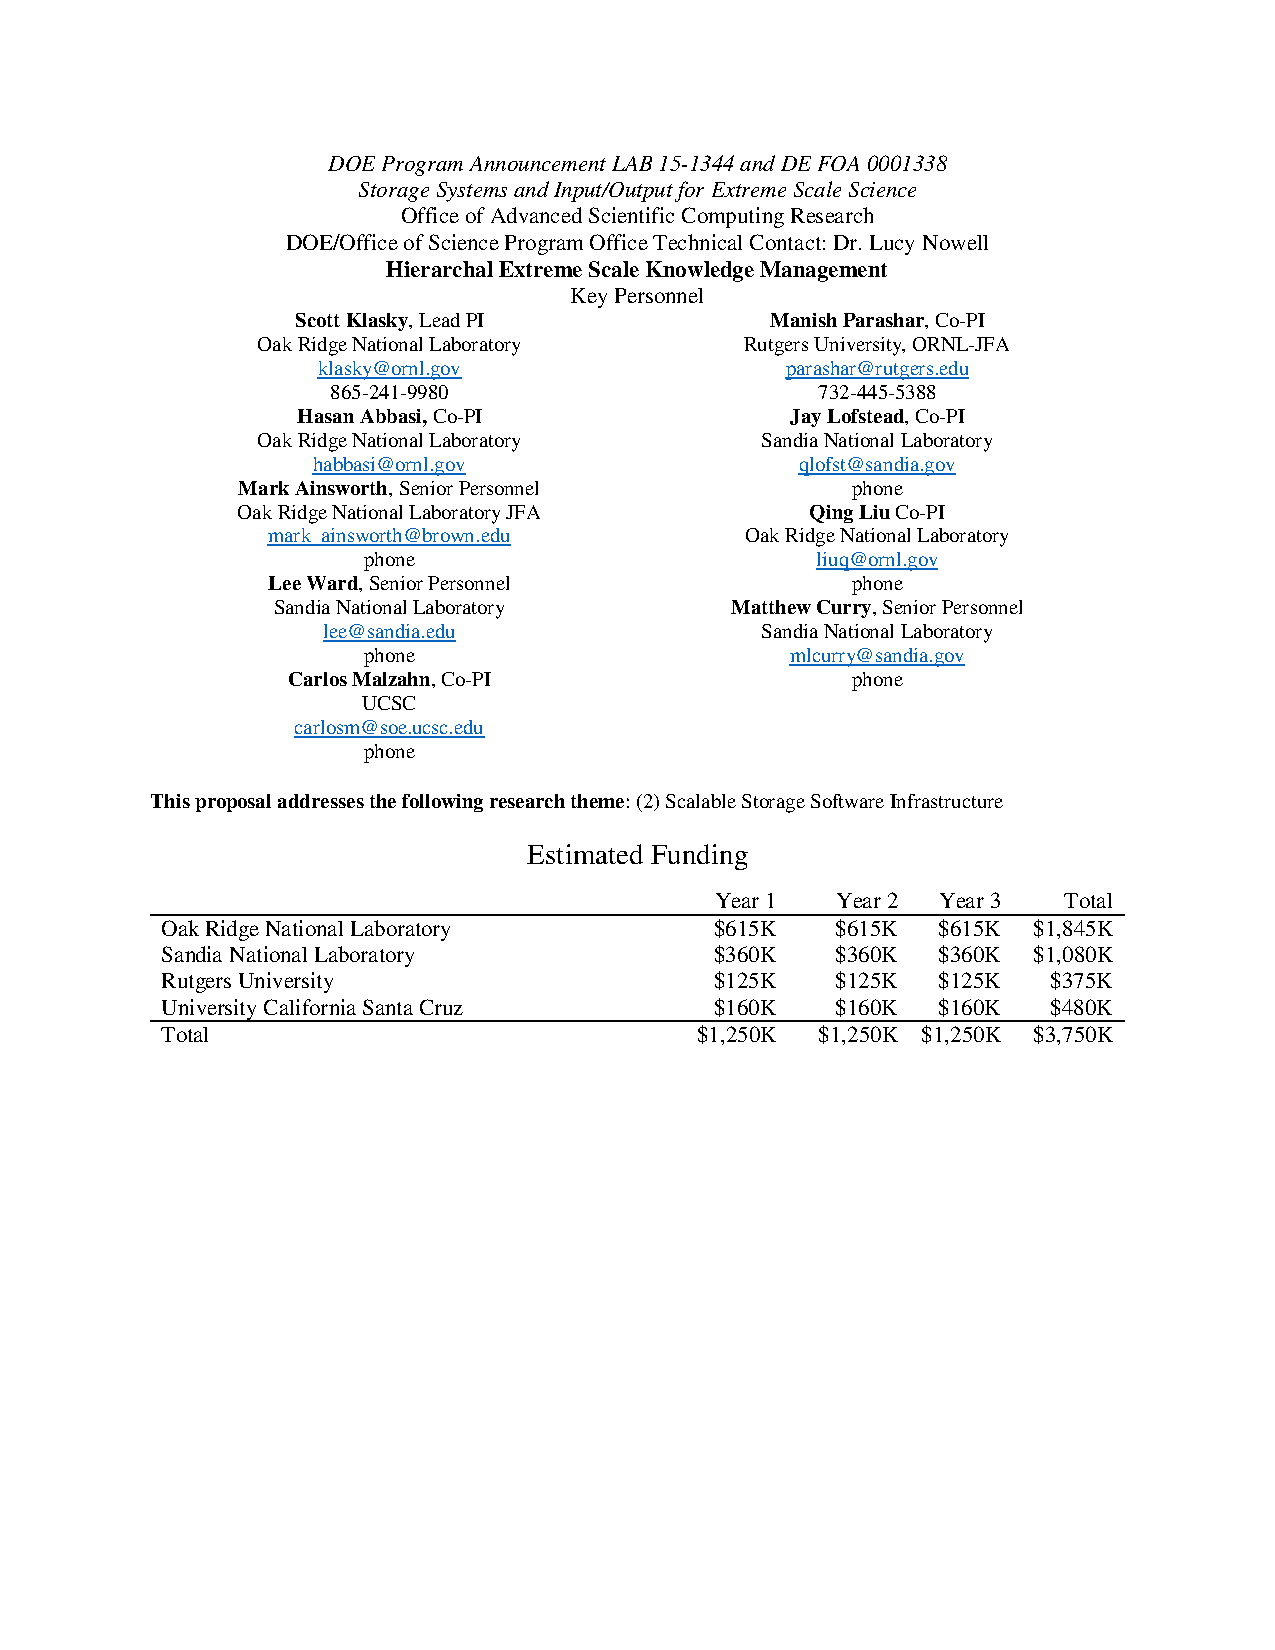
\includepdf[pages={1}]{ornl-cover.pdf}
  %  \pagebreak

\author{
  \IEEEauthorblockN {
    PI: Scott Klasky, % \IEEEauthorrefmark{1},
    Co-PI Manish Parashar % \IEEEauthorrefmark{1}
  }
  \IEEEauthorblockA {
    % \IEEEauthorrefmark{1}
    Mathematics and Computer Science Division,
    Argonne National Laboratory,
    Argonne, IL, USA}
}

%  \maketitle

  %  Heilmeyer Points: from http://www.csee.umbc.edu/~finin/home/heilmeyerCatechism.html
  %  
  %  \begin{enumerate}

  %  \item What is the problem, why is it hard? 

  %  \item How is it solved today?
  %    Fig A: much 

  %  \item What is the new technical idea; why can we succeed now?
  %    Integration of proven components into an architecture that solves
  %    problems. New research will resolve remaining technical hurdles.

  %  \item What is the impact if successful?
  %    Users and developers will be able to ...

  %  \item How will the program be organized?
  %    Participants and focus areas

  %  \item How will intermediate results be generated?
  %    Toolkit snapshots and application

  %  \item How will you measure progress?
  %    Provide metrics

  %  \item What will it cost?
  %    Cover sheet

  %  \end{enumerate}
  %   
\setlength{\parindent}{0cm}
{\bf Title of Pre-application:}  Extreme Scale Hierarchal Knowledge Management \par
{\bf Principal Investigator:} Scott Klasky, Group Leader, ORNL, 854-241-9980, klasky@ornl.gov \par
{\bf Funding Opportunity Announcement Number: DE-FOA-0001338} \par
 \vskip 0.0 in
\
\begin{tabular} {ll}
 \multicolumn{2}{l}{\bf Co-PIs and Key/Senior Personnel}\\
Hasan Abbasi, ORNL  & Mark Ainsworth, ORNL JFA, Brown University \\
Matthew Curry, SNL & Qing  Liu, ORNL \\
Jay Lofstead, ORNL & Kimmy Mu, ORNL \\
Carlos Malzahn, U. Cal. Santa Cruz & Manish Parashar, Rutgers University, ORNL JFA \\
Feiyi Wang, ORNL & Lee Ward, SNL
\end{tabular}


\setlength{\parindent}{0.5cm}

\vskip 0.1 in


\underline{\textbf{Objectives:}} Exascale scientific discovery will be
severely bottlenecked without sufficient new research into managing and
storing the large amounts of data that will be produced during the
simulation, and analyzed for months afterwards.  Our goal in this project is
to address the associated I/O and storage challenges in the context of
current and emerging storage landscapes, and expedite insights into mission
critical scientific processes. To that end, we will build on the
capabilities offered by ADIOS and DataSpaces at ORNL that provide I/O abstractions
and services, the Sirocco peer-to-peer file system at
Sandia and the object storage and annotation expertise of UC Santa Cruz, to
explore application and multi-tier storage aware data management
solutions.    This project
brings together a  team with strong expertise in I/O middleware (ORNL, Rutgers), file system (SNL, UCSC) and storage (UCSC), and connects and
coordinates these key storage components in a seamless fashion.

Our objective here is to reduce the time to knowledge, not just for a single
application, but for the entire workload in a multi-user environment, where
the storage is shared among users.
We achieve this goal by allowing selectable data quality, by trading its accuracy and error
in order to meet the time or resource constraint. 
We will explore beyond the traditional high volume I/O pattern of
checkpoint/restart, and will address the challenges posed by other essential
data access patterns in the knowledge gathering process.
Ultimately, we will take the knowledge from the storage system to provide vital feedback to the middleware 
so that the best possible decisions can be autonomically made between the user intentions and
the available system resources.  
We will test our prototypes  on current and future DOE system with many of today's applications, including the
s XGC1, GTC, QMCPack, and SpecFM3D simulations. 

Our solutions will provide novel functionalities and APIs for
\setlength{\parindent}{0cm}
%
1) specifying, at the application level, data annotations that enable the
quantification of the relative importance and utility of data objects and
enable partitioning of objects across the storage hierarch;
%
2) specifying selectable performance/quality/cost tradeoffs from both the
application and system perspectives;
%
3) evaluating these tradeoffs at runtime during data placement and movement,
and executing the resultant policies in an autonomic system using models,
heuristics and continuous learning; and
%
4) leveraging techniques such as application-aware data compression, 
%re-computation at the requisite level of accuracy, 
and I/O prioritization to enforce these
policies.
%  2) a selectable performance/quality tradeoff when reading data, and
  %  the ability to recompute data if needed, and
  %  3) incorporate reader prioritization for data annotation, placement, and data
  %  quality when writing data.  
  
  \setlength{\parindent}{0.5cm}
  
 %% Manish: Commented this since it seems to be replicated below.  
%  Our objective here is to reduce the time to knowledge, not just for a single
%application or workflow, but for the entire workload in the system. This is
%an end-to-end system wide metric relevant to the scientific discovery
%process. We will explore beyond the traditional I/O pattern of
%checkpoint/restart, and will address the challenges posed by other essential
%data access patterns in the knowledge gathering process.  Through a deeper
%insight into the scientific process we will encode and utilize accuracy and
%errors as optimization parameters.  
%Finally, we will take the knowledge from the storage system to provide vital feedback to the middleware 
%so that the best possible decisions can be autonomically  between the user intentions and
%the available system resources. Our overall goal is to ensure that optimizations can be made across
%1) a single application, 2) an ensemble of applications, and 3) the entire suite of applications which are running on the system.


  \setlength{\parindent}{0.5cm}






 % For example, scientific simulations
%contain approximations, as do measurements from observations and
%experiments, and depending on the goal, these approximations are
%acceptable. We can leverage this observation to optimize the presentation of
%data to the user and to implement various tradeoffs -- users can ask for
%information within a given accuracy bound, allowing us to offer a tradeoff for
%re-computation vs. data storage and retrieval.




%  
% \TODO{\bf: please list other things from OLCF}
% 


\underline{\textbf{Key Technical Approach:}}

Our technical approach is based on the insight that storage system awareness
of application data requirements provides a powerful tool for guiding key
extreme scale challenges such as data access method,  data representation in
storage, and data
placement within the hierarchy.
%Our overall technical approach is based on an application-aware runtime
%realization of tradeoffs in data representation, data placement and data
%access. 
Towards this goal, we will allow users, both the developers of applications
and science users running these applications, 
 to plug-in their knowledge 
about the data, represented not as bytes but as motifs, allowing the I/O and 
storage system to understand user
intentions, the relationships between data objects, as well as data access
and transport patterns. This will facilitate efficient mapping of data from
user space onto multiple storage tiers, and enable application-guided
data reductions/transformations to address capacity and bandwidth
bottlenecks. 
%
%Our approach can be most easily understood by considering a traditional
%  supermarket logistics problem. Given a limited amount of shelf space,
%  fluctuating user demands and priorities, and the need to optimize profit at
%  a market wide level instead of per product, the logistical problem combines
%  predictions about the variants and the indicated constraints to find a
%  solution. Self space is itself not a homogenous, with different locations
%  providing greater rewards to the placed items. Furthermore, haphazard
%  organization of items produces suboptimal results because it would ignore
%  locality in purchasing. Backroom and warehouses represent tiers of storage
%  where objects can be stored in bulk, but have a substantial overhead (and
%  thus lower utility) in access. Similar to this scenario, the data management
%  problem is a complex logistics problem. Shelf space is analogous to high
%  performance/lower capacity storage. Locality is an important consideration,
%  not just for single data objects but also through the identification of
%  domain meaningful relationships between objects. The tiers of the storage
%  hierarchy provide lower cost for data storage, but also increase the
%  overhead for access.
%
 For example, based on user and application insights into how the data is used,
we will offer a coarse grained, quick overview of a data set with progressively more detail in 
areas of interest such as those with features, and less detail in areas
without. These progressively more detailed data views require more storage
space and time to retrieve if left unmanaged. By defining mechanisms for applications to provide this 
knowledge and incorporating its awareness into the middleware and storage,
we will be able to selectively store data at different levels, and allow a user to select 
not only what data to retrieve but also specify an acceptable timeframe and accuracy.
On the other hand, the storage system layer may also dynamically 
adjust the level of data that will be retrieved
for an individual application, if that's allowed, to maximize the overall system efficiency and 
provide fairness among applications.

%The user may also specify guidelines that are funneled through the I/O middleware and 
%provide advice on how to react if the timeframe and error bound cannot be accepted.

%\hasan{Since we are laying the foundation for a real storage system we can't
%  be solving the problem for a single application. We will eventually have
%  to consider things like fairness, availability and this is also why we
%  want to tie in with the resource management system} 

% Our proposed I/O and storage system prototype will enable
% highly flexible data access modes that are common in scientific applications
% and associated analysis.
%
%\hasan{Can we actually take some lower accuracy representation of data (low
%  granularity MR for example, and compute more stuff to provide a higher
%  accuracy representation? I am thinking of the work with Varis Carey with
%  storing boundary state instead of full volume and then using those
%  boundaries to fill in blanks over temporally changing data}
%
The proposed work will address the following technical areas;
\\\textbf{First}, the storage system will offer the ability to directly store
different versions of a single variable to different
levels of the storage hierarchy and allow each version to be processed 
differently. For example, full data can be queued to tape while
a highly compressed version intended for high-level analytical views can be
stored in non-volatile memory (NVM) or even RAM within the storage
hierarchy. 
The key challenge here would be defining and maintaining the metadata
connecting different object quality and utility levels, 
The storage system will support the metadata and plug-ins required to support
this data storage approach.   
%data re-computation is allowed to re-generate data with
%customizable accuracy, if the associated computing and I/O cost is lower
%than retrieving the target data from a {\em slow} tier.
%
\textbf{Second}, new storage access APIs will be developed that incorporates the
notion of time and data quality for requested data. The storage system,
through the knowledge of both data quality stored in different storage
hierarchy tiers and the approximate time to retrieve data from the different
tiers, can manage (with the user in the loop) the tradeoff between error bound and the time to
retrieve data. This storage system support will be executed and managed through our middleware, 
insulating the user as much as possible from the new APIs. The storage system
will also support plug-ins, for example, to potentially decompress or expand data to the
original size. Both lossless and lossy with error bounds style storage is
assumed. The time factor must take into account how long this operation takes
for servicing the user request. 
%exploratory analysis operations frequently entail an
%overall data set view followed by targeted data exploration on extracted
%features.  In particular, the {\em overview} access mode gives a quick but
%approximate data view that can guide feature selection offering rapid
%coarse-grained data exploration without requiring loading the high-accuracy
%data from storage. Based on the granularity requested, the accuracy and size
%of the data returned can be adjusted. In the most extreme setting, the
%original data can be retrieved at the time cost of moving the potentially
%huge data quantity.
%
\textbf{Third}, the storage system will offer annotations within the metadata
and support for both predictive and reactive data placement and migration.
While past access patterns may not indicate future access because the
simulation details may have changed, we are focused on scalability where
subsequent runs are larger in scale as the simulation prepares for a capability run.  By
learning from the output and access patterns during this run sequence, we can
accurately decide how to place and organize data for the critical capability
runs. The reactive mechanisms will consider the space and performance
characteristics, as well as the requested data fidelity, to determine where and
how to pull and store data sets. The challenge here is to utilize this
metadata to manage the placement and access of data object based on the
defined constraints as well as storage system state. 

% In some cases, a full fidelity dataset may be pulled
% from tape to disk and no further to preserve 100\% data fidelity. In others, a
% lossy-compressed within error bounds version may be generated and stored in
% local node RAM for very fast access with an acceptable error.
%to ensure available storage for subsequent operations, we
%will offer automatic data migration, based on user annotations for required
%data and using monitoring and learning techniques.  Unlike existing
%approaches, this will be driven both by the user annotations and through
%learned access patterns in
%an autonomic and crosslayer manner.
%
\textbf{Fourth}, to effectively manage data storage capacities, the storage
system's capability for storing multiple, potentially different data quality
versions of the same data will be leveraged to guide data eviction and migration. 
The main challenge of this approach is to be aware of intentional placement
decisions made to optimize future data access while ensuring proper system
operation by not exhausting any tier inappropriately. If a single application
has been allocated the entire machine for a capability run, completely
consuming resources on the machine is expected. For smaller runs, these
allocations must be balanced to support the diverse workload. 
Our research efforts will be heavily focused on the need to, in a
coordinated manner, adapt data and metadata retention policies according to the 
dynamic resource balancing that will need to take place between the
application, OS/R, and hardware.

%we anticipate storing multiple data copies, each compressed
%in different ways according to the underlying media, some of these copies
%will disappear based on storage pressures, but data persistence will be
%maintained according to user specifications. Assuming a relatively low
%latency cache layer before a tape system, we can offer exploratory data
%access reserving pulling data from tape to just the data required. 
% Additionally, we will incorporate data life time, at sub-object
%granularity, as a user described metric to allow the storage system to
%intelligently make decisions on purging and evicting data. 

 
% A key challenge in this project is defining and maintaining the metadata
% connecting different object quality and utility levels, and using this metadata 
% to most appropriately manage the placement and access of data object based on 
% user/application intent/constraints and storage system state.
% %The new user APIs required to interact with this rich metadata system will
% %drive effective use of the entire middleware and storage stack.
% Our research efforts will be heavily focused on the need to, in a
% coordinated manner, adapt data and metadata retention policies according to the 
% dynamic resource balancing that will need to take place between the
% application, OS/R, and hardware.

The success of this project will provide insights into how to build extreme scale
autonomic middleware and storage layers that can interact effectively with each
other, and bring the user in the loop through user-provided hints, allowing user 
and system knowledge to be incorporated into the SSIO software layers.
Storage resources will be managed against the needs of individual simulations 
as well as what's happening on the entire system. The impact of such a solution 
will be a significant reduction in the time to knowledge, and the overall increase in 
the effectiveness and utility of exascale simulations.

%Today, data is reduced by application
%scientist who have limited information on what the storage layer can
%provide. 

%They often make compromises based on this limited knowledge and
%either tune their output for writing or reading performance. This data then
%gets moved to other locations, and much of the tuning is lost when the data
%is read back during their post processing. Furthermore, there is a limited
%set of operations which users will be able to stage to other staging nodes
%for real-time-reduction and visualization.


%  \includepdf[pages={1}]{COI.pdf}

\end{document}

%%% End: 

%%% Local Variables:
%%% mode: latex
%%% TeX-master: t
%%% End:
